%\documentclass[twocolumn]{article}
%\usepackage[utf8]{inputenc}
%\documentclass[10pt,journal,onecolumn]{IEEEtran}
%\documentclass[10pt,journal,compsoc]{IEEEtran}
\documentclass[10pt, journal, letterpaper]{IEEEtran}
%\documentclass[10pt,journal,compsoc]{IEEEtran}


% NB hyperref package may need to be commented for Latex upload
\usepackage{cite}
%\ifCLASSOPTIONcompsoc
%\ifCLASSINFOpdf
% \usepackage[pdftex]{graphicx}
% declare the path(s) where your graphic files are
% \graphicspath{{../pdf/}{../jpeg/}}
% and their extensions so you won't have to specify these with
% every instance of \includegraphics
% \DeclareGraphicsExtensions{.pdf,.jpeg,.png}
%  \usepackage[nocompress]{cite}
%  \else
% normal IEEE
%  \usepackage{cite}
%  \fi

%  \ifCLASSINFOpdf

%  \else
%\fi
%important package
\usepackage{multirow} 
\usepackage{algpseudocode}
\usepackage{algorithm}
\usepackage{rotating}
\usepackage{kantlipsum} %with the next two command (commath, allowdisplaybreaks) -> allow to break the formulas along the pages
\usepackage{commath}
\allowdisplaybreaks
\usepackage{mathtools}  %with the next command adjust the vertical space between formulas
%\setlength{\jot}{5pt}
%\usepackage{ragged2e}   %if add \justify at each line, that line would be justified. This is used because the abstract of transaction style is not justified  ---- it is not compatible with twocolumn-IEEETrans
%not important
\usepackage{verbatim}
\usepackage{xr-hyper} 
\usepackage{enumitem}
\usepackage{multirow}
\usepackage[table,xcdraw]{xcolor}
\usepackage{array,arydshln}
\usepackage{graphicx,booktabs}
\usepackage{longtable}
%strikethrough not working when nested in a definition
%\usepackage[normalem]{ulem}
%\usepackage{soul}
%\usepackage{fullpage} 
%%%%%%%%%%%%%%%%%%%%%%%%%%%%%%%%%%%%%%%%%%%%%%%%%%%%%%%%%%%%%%%%%%%%%%%%%%%%%
% hyperref package may need to be commented for Latex upload
%\usepackage[pdfusetitle, pdfauthor={Michael Shell, My institution}]{hyperref}
%%%%%%%%%%%%%%%%%%%%%%%%%%%%%%%%%%%%%%%%%%%%%%%%%%%%%%%%%%%%%%%%%%%%%%%%%%%%%
\usepackage{balance}
\usepackage{flushend}
\usepackage{epstopdf}
\usepackage{wrapfig}
\usepackage{latexsym}
\usepackage{amssymb}
\usepackage{amsthm}
\usepackage{amsfonts}
\usepackage{amsmath} %[cmex10]
%\usepackage{flushend} %********************* This package has a bug: Do no include it
\usepackage{graphicx}
\usepackage{latexsym}
\usepackage{booktabs}
\usepackage[style=base]{caption}
\usepackage{subcaption} %******************* This package has conflict with sufig and subfigure
%\usepackage{subfigure}
%\usepackage{subfig}
\usepackage{breqn}
\newtheorem{thm}{Property}
\newtheorem{thm1}{Theorem}
\newtheorem{thm3}{Proposition}
\newtheorem{thm5}{Remark}
\newtheorem{thm7}{Lemma}
\algnewcommand\algorithmicinput{\textbf{INPUT:}}
\algnewcommand\INPUT{\item[\algorithmicinput]}
\algnewcommand\algorithmicoutput{\textbf{OUTPUT:}}
\algnewcommand\OUTPUT{\item[\algorithmicoutput]}
\usepackage[table]{xcolor}
%\usepackage[dvipsnames]{xcolor}
%\usepackage[cmyk]{xcolor}
%\usepackage{natbib}
\usepackage{graphicx}
\usepackage{mathtools}
\usepackage{enumitem,kantlipsum}
\usepackage{adjustbox}
% change the width and height of rows and columns in Tables
\usepackage[thinlines]{easytable}

\algdef{SE}[DOWHILE]{Do}{doWhile}{\algorithmicdo}[1]{\algorithmicwhile\ #1}
\makeatletter
\algnewcommand{\LineComment}[1]{\Statex \hskip\ALG@thistlm \texttt{#1}}
\makeatother
\newcommand{\export}{Exportation\xspace}
\newcommand{\move}{Move\xspace}
\newcommand{\ouralgorithm}{GPE\xspace} %%Green path exportation

\newlength\mylength
\setlength\mylength{\dimexpr.13\columnwidth-1\tabcolsep-0.2\arrayrulewidth\relax}
\usepackage{color}
% we need a better fix for this, see https://tex.stackexchange.com/questions/64298/error-with-xcolor-package
\colorlet{BLUE}{blue}
\usepackage{colortbl}
\definecolor{LightCyan}{RGB}{155, 227, 247}
%\captionsetup[figure]{belowskip=-8pt}
%in test

%\usepackage{nomencl}
%\makenomenclature
%% This code creates the groups
% -----------------------------------------
%\usepackage{etoolbox}
%\renewcommand\nomgroup[1]{%
%	\item[\bfseries
%	\ifstrequal{#1}{P}{Parameters}{%
%		\ifstrequal{#1}{V}{Variables}{%
%			\ifstrequal{#1}{I}{Indices}{%
%				\ifstrequal{#1}{B}{Binary~Variables}{}}}}%
%	]}

%DOUBLE QUOTATION COMMAND
\newcommand{\dq}[1]{``#1''}

% To remove all comments, comment out the definition and use the commented-out
% empty definition below
% otherwise you can comment the line \commentsontrue 
\newcommand{\commentBy}[3]{\textcolor{#1}{\textbf{#2:} #3}}
%\newcommand{\commentBy}[3]{\ignorespaces}

\newif\ifcommentson
%uncomment the line below to show comments
\commentsontrue

\newcommand{\ste}[1]{\ifcommentson \commentBy{blue}{SS}{#1} \fi}
%\newcommand{\lc}[1]{\ifcommentson \commentBy{blue}{LC}{#1} \fi}
\newcommand{\mm}[1]{\ifcommentson \commentBy{orange}{MM}{#1} \fi}

\newif\ifextended
\newif\ifshortver

%%% Show only short version in black
%%%        \shorvetrue 
%%%        %\extendedtrue 

%%% Show only extended version in black
%%%        %\shorvetrue 
%%%        \extendedtrue 

%%% Show short version in blue and extended version in purple
%%%        \shorvetrue 
%%%        \extendedtrue 

\shortvertrue
%\extendedtrue

\newcommand{\extended}[1]{\ifextended \ifshortver \textcolor{purple}{#1} \else \textcolor{black}{#1} \fi  \fi}
\newcommand{\shortver}[1]{\ifshortver \ifextended \textcolor{blue}{#1} \else \textcolor{black}{#1} \fi \fi}

%\newcommand{\optional}[1]{#1}
%\newcommand{\optional}[1]{\textcolor{Orange}{#1}}
\newcommand{\optional}[1]{\ignorespaces}


\newif\ifrevisionactive
\newif\ifshowdeleted
\revisionactivetrue
%\showdeletedtrue

\newcommand{\revised}[1]{\ifrevisionactive \textcolor{blue}{#1} \else \textcolor{black}{#1} \fi}

%\newcommand{\deleted}[1]{\ifrevisionactive \ifshowdeleted \textcolor{red}{\sout{#1}} \else \fi \fi}
\newcommand{\deleted}[1]{\ifrevisionactive \ifshowdeleted \textcolor{orange}{#1} \else \fi \fi}


% correct bad hyphenation here
\hyphenation{net-works mo-ni-to-ring par-ti-cu-lar pe-ri-o-di-cal-ly mi-ni-mi-zing va-ria-tions de-li-ve-red per-ri-o-di-cal-ly}


\newcommand\linearFigSze{0.48}
\newcommand\histFigSze{0.48}
\newcommand\boxFigSze{0.7}

\begin{document}
% \title{Active Monitoring for Virtual Networks: Real-Time Delay Measurement for SDN-based Networks}
\title{Active Delay Measurement for SDN-based Networks}
\author{}
%\date{October 2018}
\maketitle	
\begin{abstract}
\end{abstract}	
\begin{IEEEkeywords} 
    Passive Network Monitoring;
\end{IEEEkeywords}

\section{Introduction}

\section{Network Throughput}

\subsection{Flow per Second and bit per Second}
Dashed lines show the lockdowns of different countries in Europe. %Worldwide curfews, quarantines, and similar restrictions were in place to prevent the further spread of COVID-19.
Countries and territories around the world have enforced lockdowns of varying degrees. Some include total movement control while others have enforced restrictions based on time. Mostly, only essential businesses are allowed to remain open.% Schools, universities and colleges have closed either on a nationwide or local basis in 161 countries, affecting approximately 98.6 per cent of the world's student population.

\begin{table}[]
    \centering
    \resizebox{\columnwidth}{!}{
    \begin{tabular}{|l|c||l|c|}\hline
        Country & Lockdown Date & Country & Lockdown Date \\\hline\hline
        Italy & 2020-03-09 & Denmark & 2020-03-11\\\hline
        Norway & 2020-03-12 & Spain & 2020-03-14\\\hline
        Austria & 2020-03-16 & Switzerland & 2020-03-17\\\hline
        Ukraine & 2020-03-17 & France & 2020-03-17 \\\hline
        Luxembourg & 2020-03-18 & Germany & 2020-03-20\\\hline
        Germany & 2020-03-21 & UK \& Greece & 2020-03-23\\\hline
        Romania & 2020-03-25 & Finland & 2020-03-27\\\hline
    \end{tabular}}
    \caption{Lock-downs}
    \label{tab:lockdowns}
\end{table}

In table~\ref{tab:lockdowns}, pandemic lockdowns are defined as the shutdown of parts of the economy, due to non-pharmaceutical anti-pandemic measures and are enforceable by law like:
\begin{itemize}
    \item Closing of schools and kindergartens
    \item Closing of non-essential shops (shops and stores apart from food, doctors and drug stores)
    \item Closing of non-essential production
    \item Cancellation of recreational venues and closing of public places
    \item Curfews
    \item Stay-at-home orders and total movement control
\end{itemize}
The table does not contain:
\begin{itemize}
    \item Measures with smaller economic impacts like:
    \begin{itemize}
        \item border closures
        \item social distancing measures and social movement restrictions
        \item travel restrictions.
    \end{itemize}
    \item Other non-pharmaceutical anti-pandemic measures like mandatory quarantines after travel, self quarantine and social distancing measures
    \item Any measures which are voluntary rather than enforceable by law 
\end{itemize}

\begin{figure*}
    \begin{subfigure}{\linearFigSze\textwidth}
          \centering
          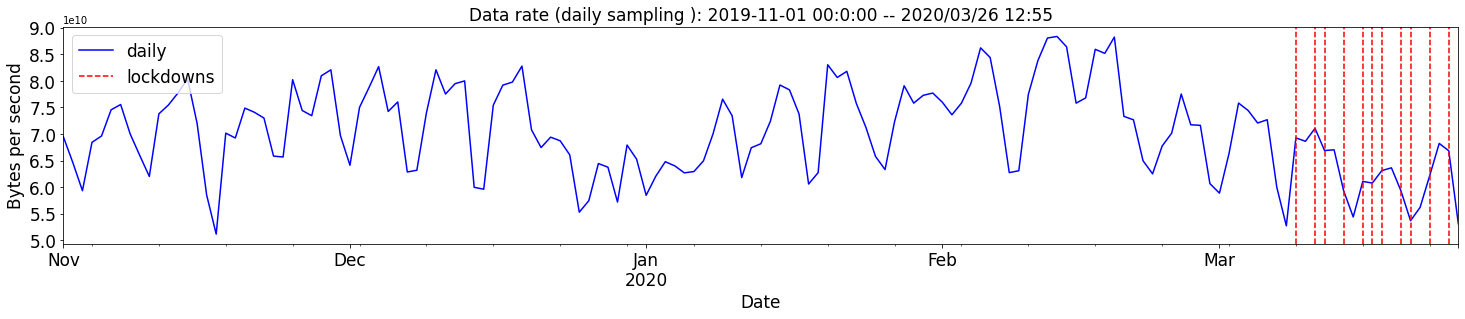
\includegraphics[width=\columnwidth]{img/traffic_trend_bps.png}
          \caption{Bytes per second}
          \label{fig:traffic_trend_bps}
    \end{subfigure}
    \begin{subfigure}{\linearFigSze\textwidth}
          \centering
          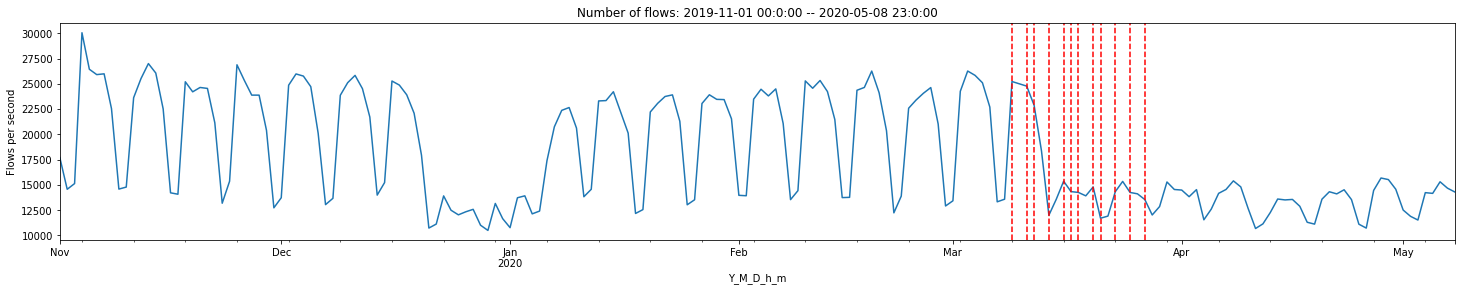
\includegraphics[width=\columnwidth]{img/traffic_trend_fps.png}
          \caption{Flow per second}
          \label{fig:traffic_trend_fps}
    \end{subfigure}
    \caption{Network Throughput}
    \label{fig:network_throughput}
\end{figure*}

The sampling of bps has faced a problem since 2020/03/26 12:55. 

\subsection{Break-down to Academic and Business}
\begin{figure*}
    \begin{subfigure}{\linearFigSze\textwidth}
          \centering
          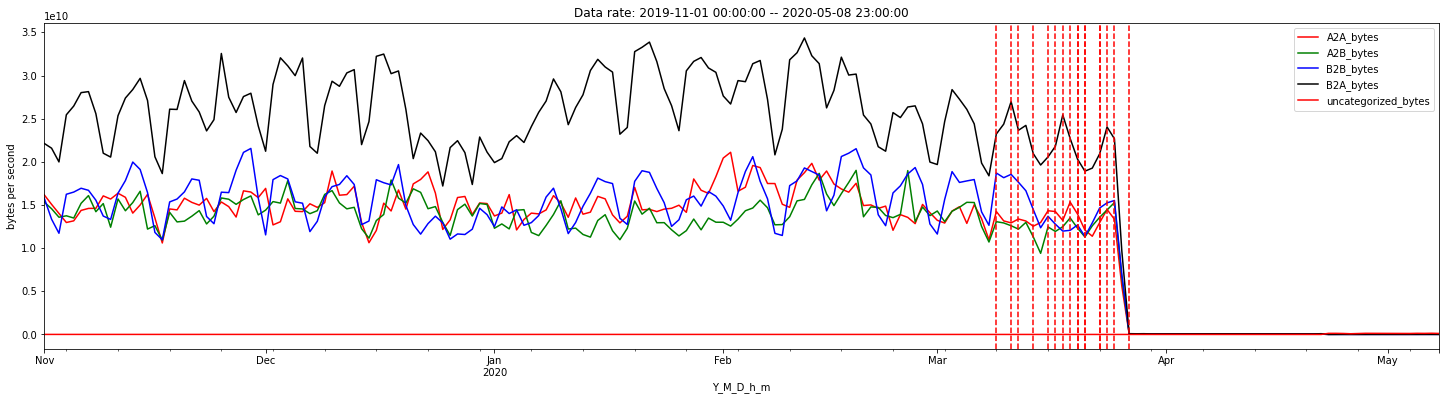
\includegraphics[width=\columnwidth]{img/traffic_trend_bps_AcaVsBus.png}
          \caption{Bytes per second}
          \label{fig:traffic_trend_acaVSbusi_bps}
    \end{subfigure}
    \begin{subfigure}{\linearFigSze\textwidth}
          \centering
          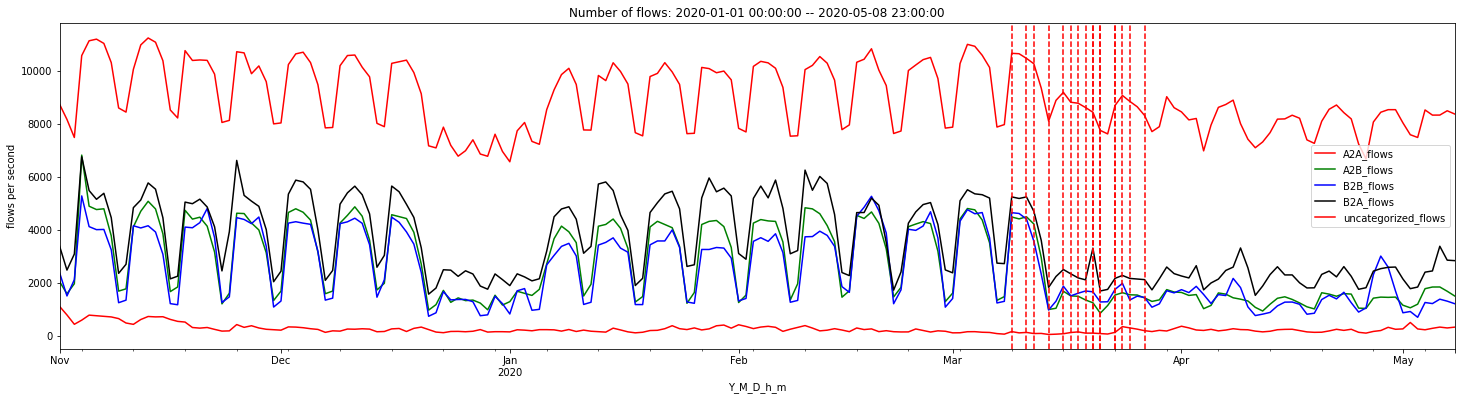
\includegraphics[width=\columnwidth]{img/traffic_trend_fps_AcaVsBus.png}
          \caption{Flow per second}
          \label{fig:traffic_trend_acaVSbusi_fps}
    \end{subfigure}
    \caption{Network Throughput Breakdown}
    \label{fig:network_throughput_breakdown}
\end{figure*}

\section{NRENs Traffic Pattern}
\subsection{fps and bps}
\begin{figure*}
    \begin{subfigure}{\linearFigSze\textwidth}
          \centering
          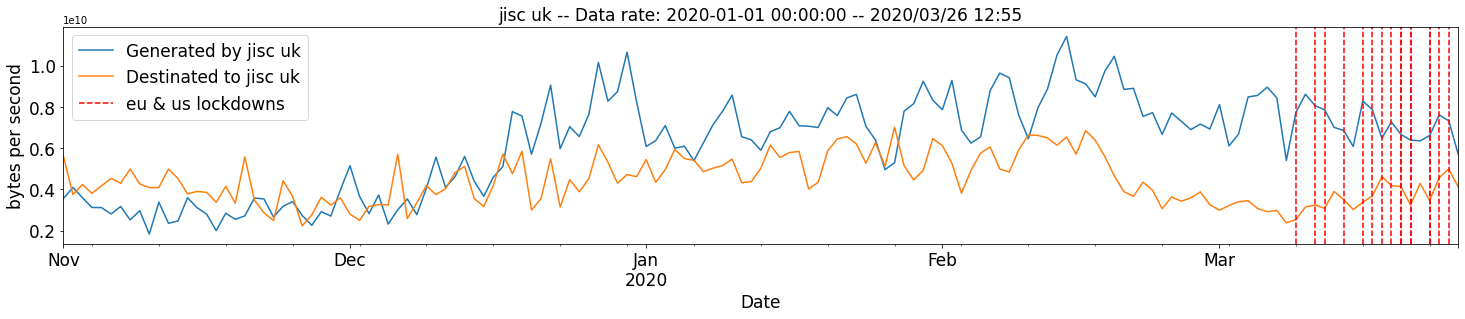
\includegraphics[width=\columnwidth]{img/jisc_bps.png}
          \caption{JISC}
          \label{fig:jisc_bps}
    \end{subfigure}
    \begin{subfigure}{\linearFigSze\textwidth}
          \centering
          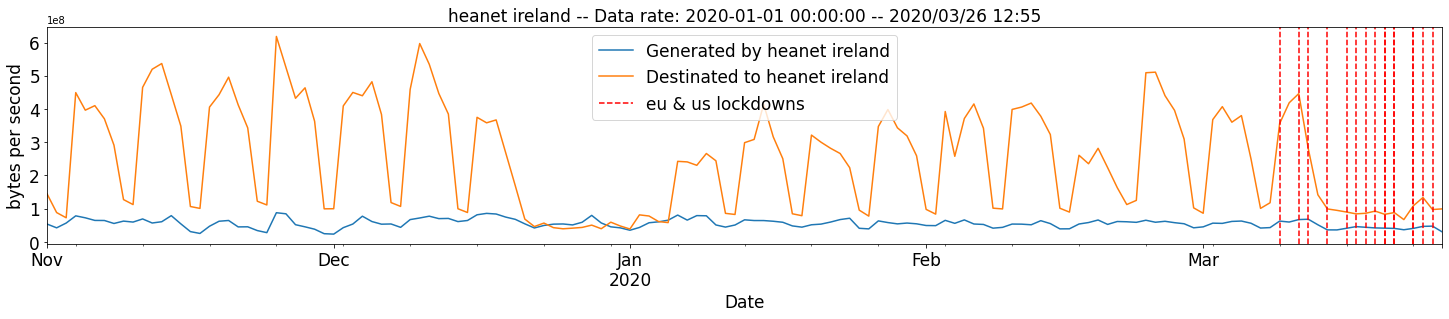
\includegraphics[width=\columnwidth]{img/heanet_bps.png}
          \caption{HEANET}
          \label{fig:HEANET_bps}
    \end{subfigure}
    \begin{subfigure}{\linearFigSze\textwidth}
          \centering
          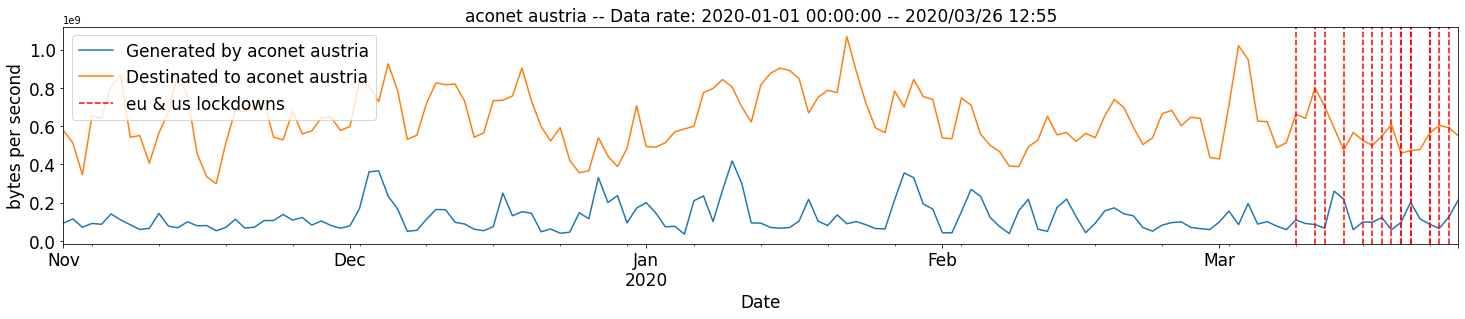
\includegraphics[width=\columnwidth]{img/aconet_bps.png}
          \caption{ACONET Austria}
          \label{fig:aconet_bps}
    \end{subfigure}
    \begin{subfigure}{\linearFigSze\textwidth}
          \centering
          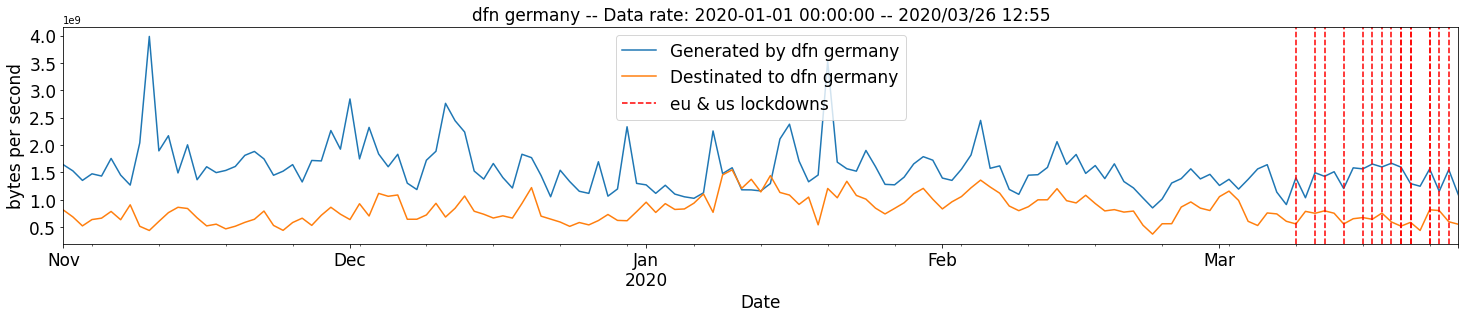
\includegraphics[width=\columnwidth]{img/dfn_bps.png}
          \caption{DFN Germany}
          \label{fig:dfn_bps}
    \end{subfigure}
    \begin{subfigure}{\linearFigSze\textwidth}
          \centering
          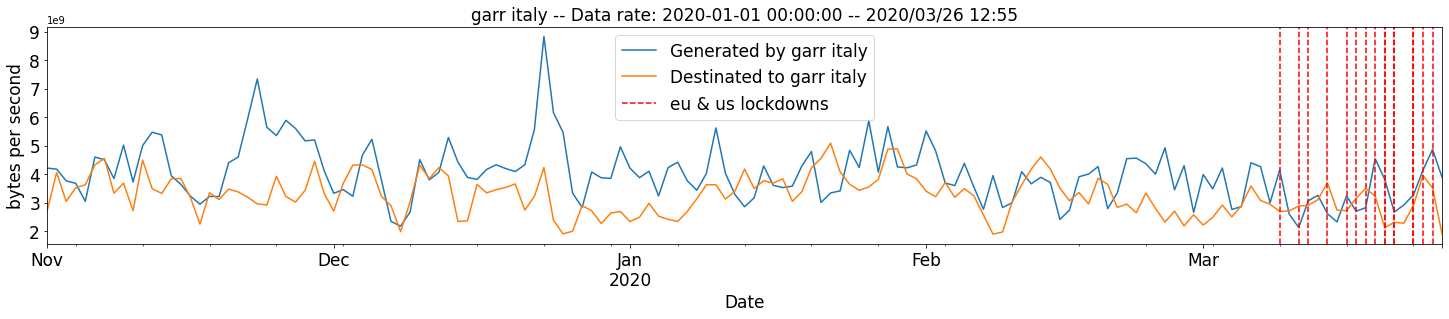
\includegraphics[width=\columnwidth]{img/garr_bps.png}
          \caption{GARR Italy}
          \label{fig:garr_bps}
    \end{subfigure}
    \begin{subfigure}{\linearFigSze\textwidth}
          \centering
          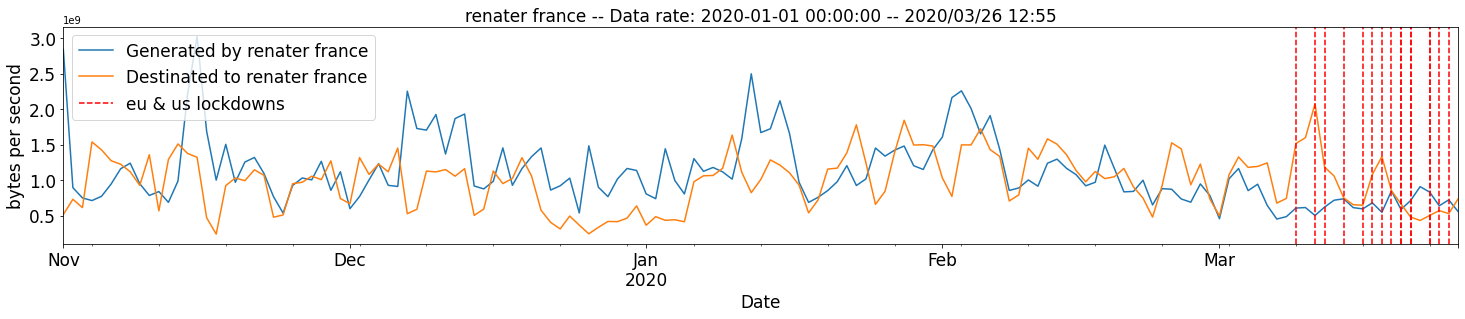
\includegraphics[width=\columnwidth]{img/rediris_bps.png}
          \caption{REDIRIS Spain}
          \label{fig:rediris_bps}
    \end{subfigure}
    \begin{subfigure}{\linearFigSze\textwidth}
          \centering
          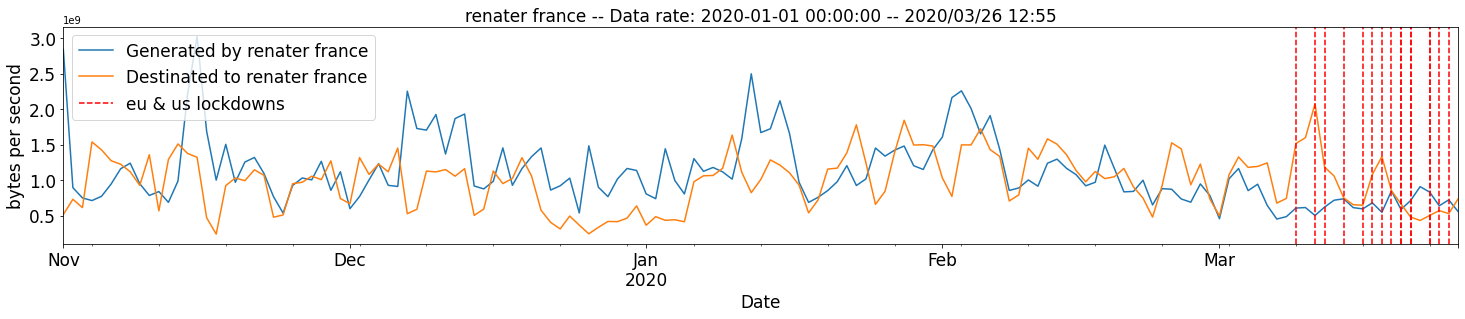
\includegraphics[width=\columnwidth]{img/renater_bps.png}
          \caption{RENATER France}
          \label{fig:renater_bps}
    \end{subfigure}
    \begin{subfigure}{\linearFigSze\textwidth}
          \centering
          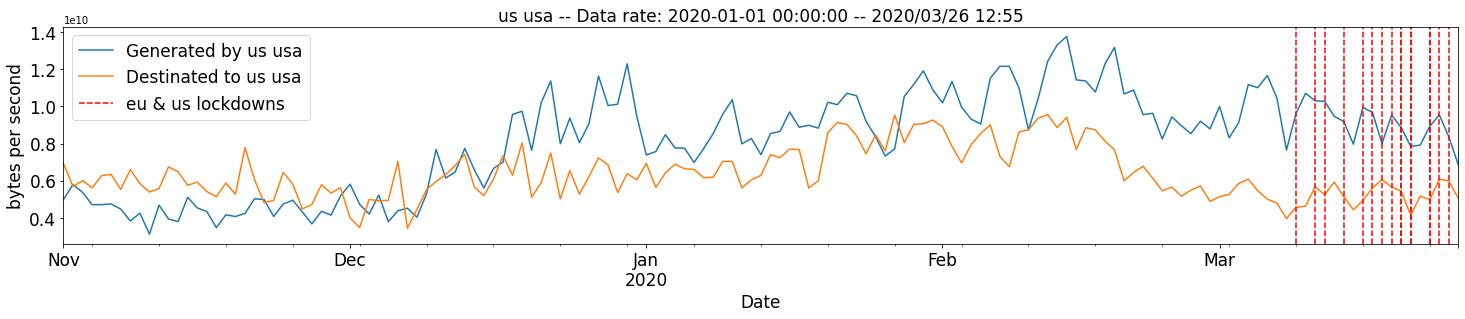
\includegraphics[width=\columnwidth]{img/us_bps.png}
          \caption{US NREN}
          \label{fig:US_bps}
    \end{subfigure}
    \begin{subfigure}{\linearFigSze\textwidth}
          \centering
          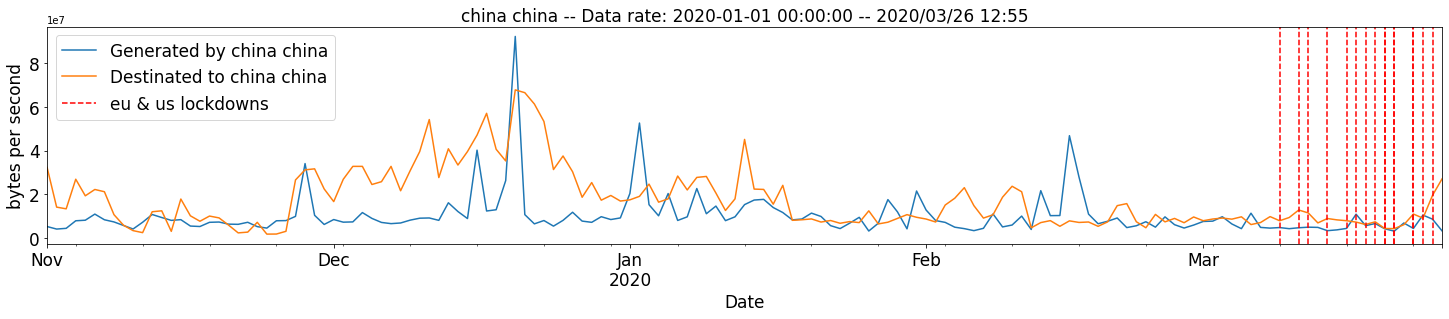
\includegraphics[width=\columnwidth]{img/china_bps.png}
          \caption{China NREN}
          \label{fig:china_bps}
    \end{subfigure}
    \caption{NRENs' Throughput (bps)}
    \label{fig:nrens_bps}
\end{figure*}
\begin{figure*}
    \begin{subfigure}{\linearFigSze\textwidth}
          \centering
          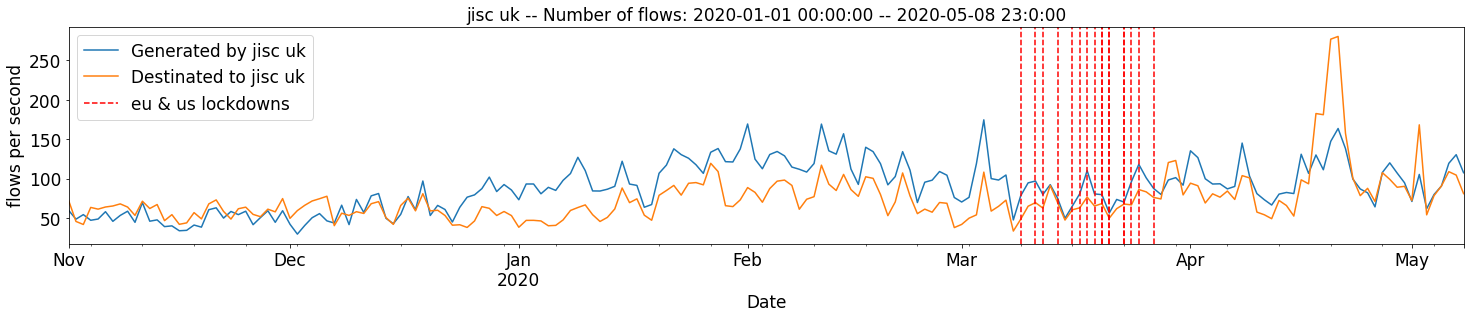
\includegraphics[width=\columnwidth]{img/jisc_fps.png}
          \caption{JISC}
          \label{fig:jisc_fps}
    \end{subfigure}
    \begin{subfigure}{\linearFigSze\textwidth}
          \centering
          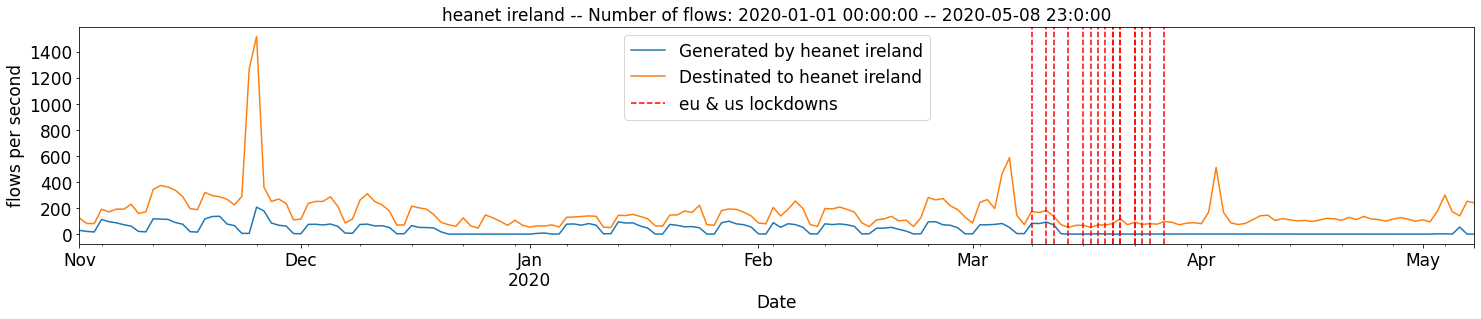
\includegraphics[width=\columnwidth]{img/heanet_fps.png}
          \caption{HEANET}
          \label{fig:HEANET_fps}
    \end{subfigure}
    \begin{subfigure}{\linearFigSze\textwidth}
          \centering
          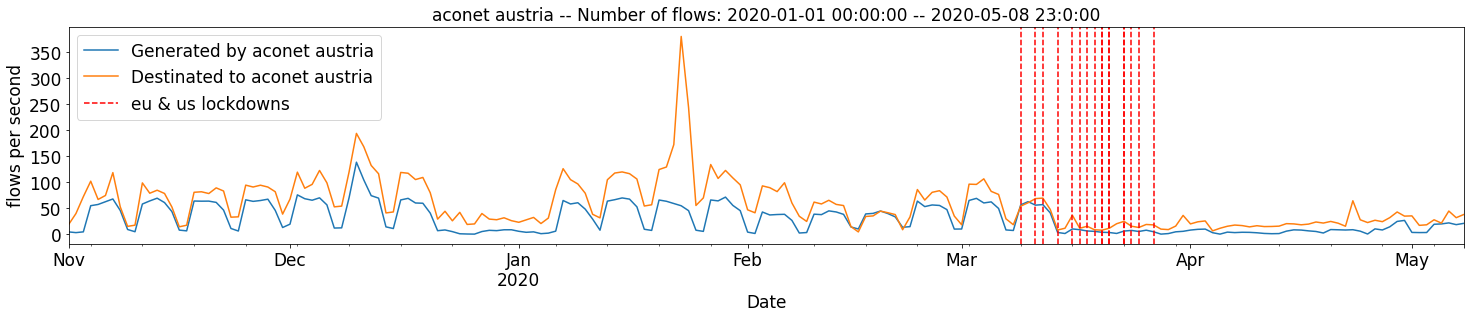
\includegraphics[width=\columnwidth]{img/aconet_fps.png}
          \caption{ACONET Austria}
          \label{fig:aconet_fps}
    \end{subfigure}
    \begin{subfigure}{\linearFigSze\textwidth}
          \centering
          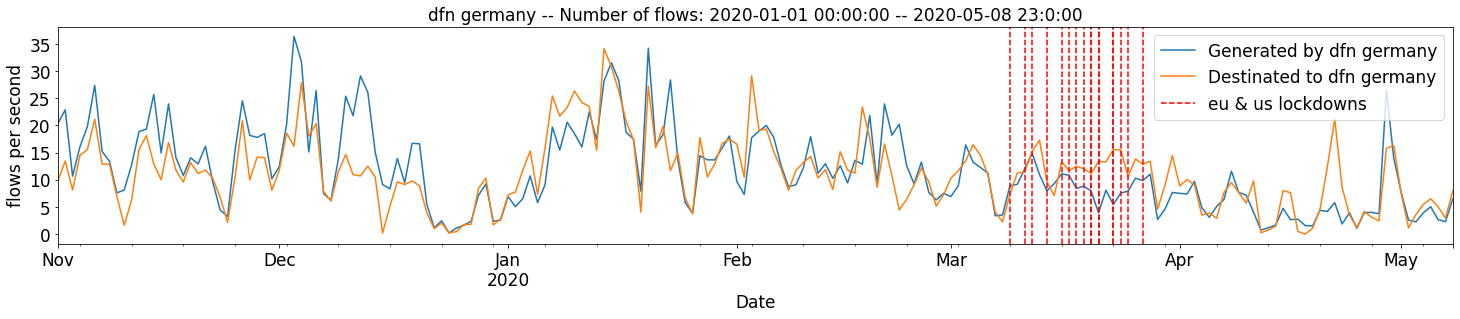
\includegraphics[width=\columnwidth]{img/dfn_fps.png}
          \caption{DFN Germany}
          \label{fig:dfn_fps}
    \end{subfigure}
    \begin{subfigure}{\linearFigSze\textwidth}
          \centering
          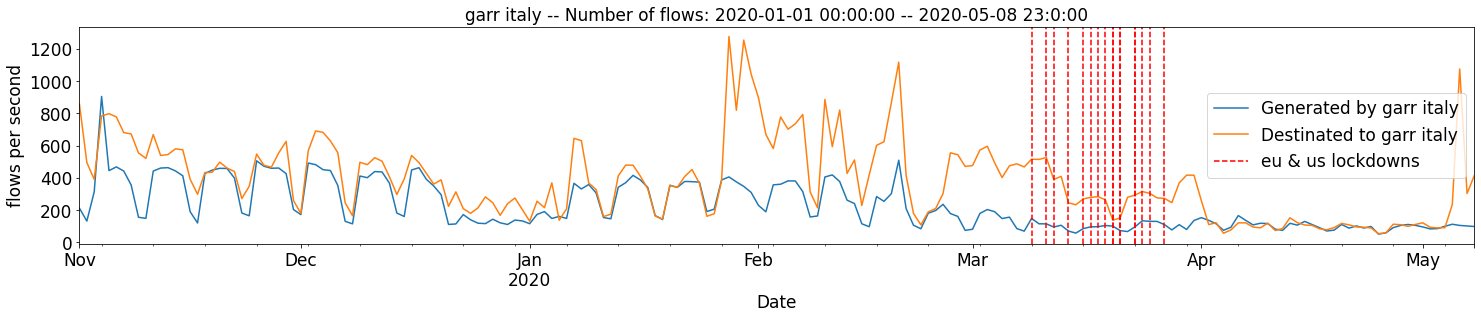
\includegraphics[width=\columnwidth]{img/garr_fps.png}
          \caption{GARR Italy}
          \label{fig:garr_fps}
    \end{subfigure}
    \begin{subfigure}{\linearFigSze\textwidth}
          \centering
          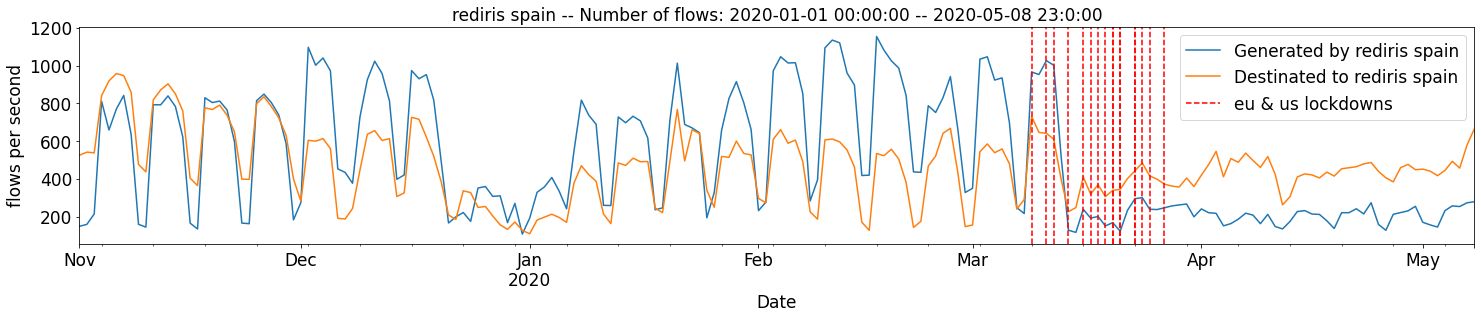
\includegraphics[width=\columnwidth]{img/rediris_fps.png}
          \caption{REDIRIS Spain}
          \label{fig:rediris_fps}
    \end{subfigure}
    \begin{subfigure}{\linearFigSze\textwidth}
          \centering
          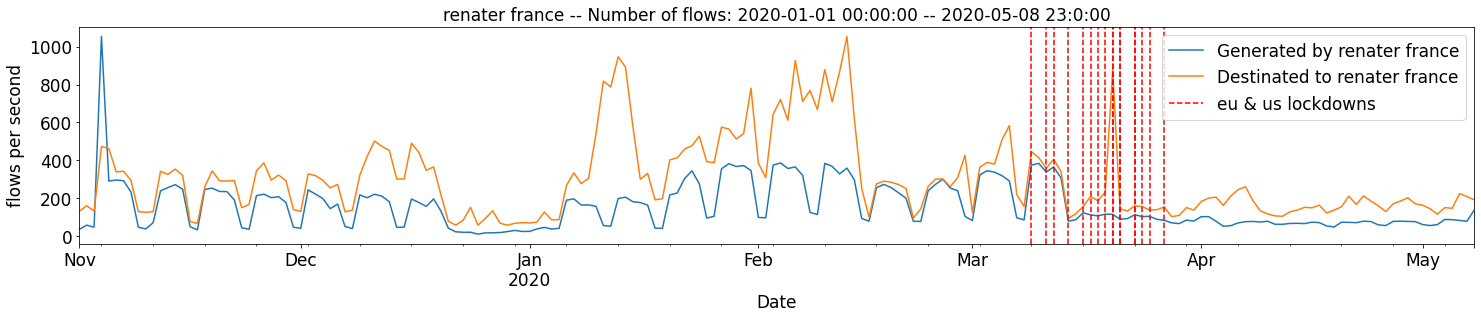
\includegraphics[width=\columnwidth]{img/renater_fps.png}
          \caption{RENATER France}
          \label{fig:renater_fps}
    \end{subfigure}
    \begin{subfigure}{\linearFigSze\textwidth}
          \centering
          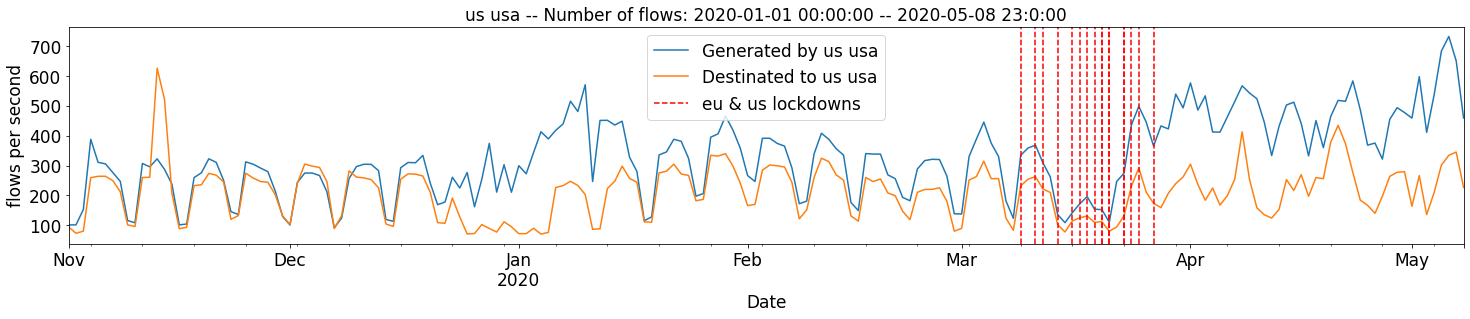
\includegraphics[width=\columnwidth]{img/us_fps.png}
          \caption{US NREN}
          \label{fig:US_fps}
    \end{subfigure}
    \begin{subfigure}{\linearFigSze\textwidth}
          \centering
          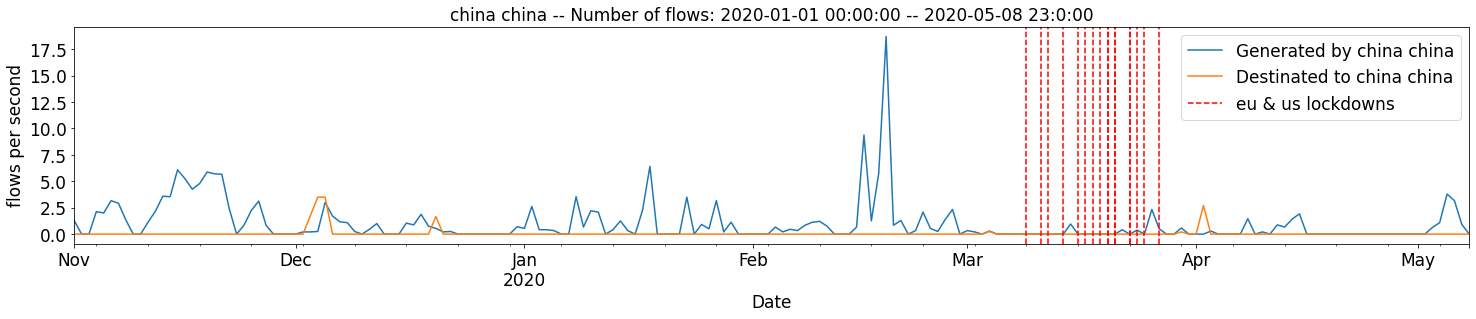
\includegraphics[width=\columnwidth]{img/china_fps.png}
          \caption{China NREN}
          \label{fig:china_fps}
    \end{subfigure}
    \caption{NRENs' Throughput (fps)}
    \label{fig:nrens_fps}
\end{figure*}

\subsection{break-down to Academic and Business}
\begin{figure*}
    \begin{subfigure}{\linearFigSze\textwidth}
          \centering
          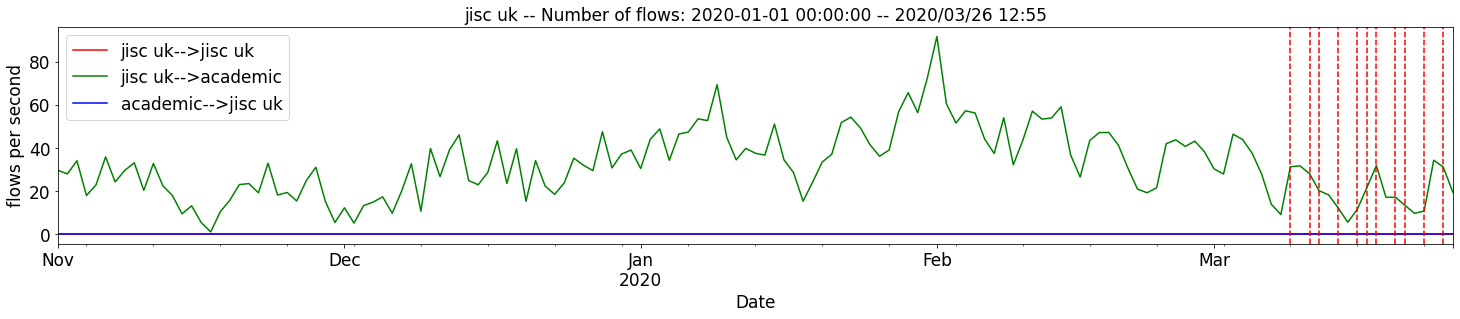
\includegraphics[width=\columnwidth]{img/jisc_aca_bps.png}
          \caption{JISC}
          \label{fig:jisc_aca_bps}
    \end{subfigure}
    % \begin{subfigure}{\linearFigSze\textwidth}
    %       \centering
    %       \includegraphics[width=\columnwidth]{img/heanet_aca_fps.png}
    %       \caption{HEANET}
    %       \label{fig:HEANET_aca_fps}
    % \end{subfigure}
    % \begin{subfigure}{\linearFigSze\textwidth}
    %       \centering
    %       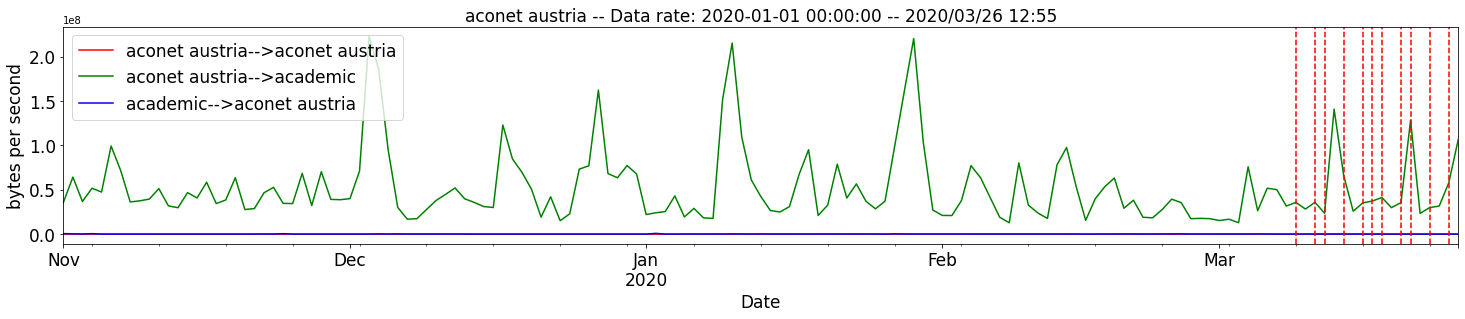
\includegraphics[width=\columnwidth]{img/aconet_aca_bps.png}
    %       \caption{ACONET Austria}
    %       \label{fig:aconet_aca_bps}
    % \end{subfigure}
    \begin{subfigure}{\linearFigSze\textwidth}
          \centering
          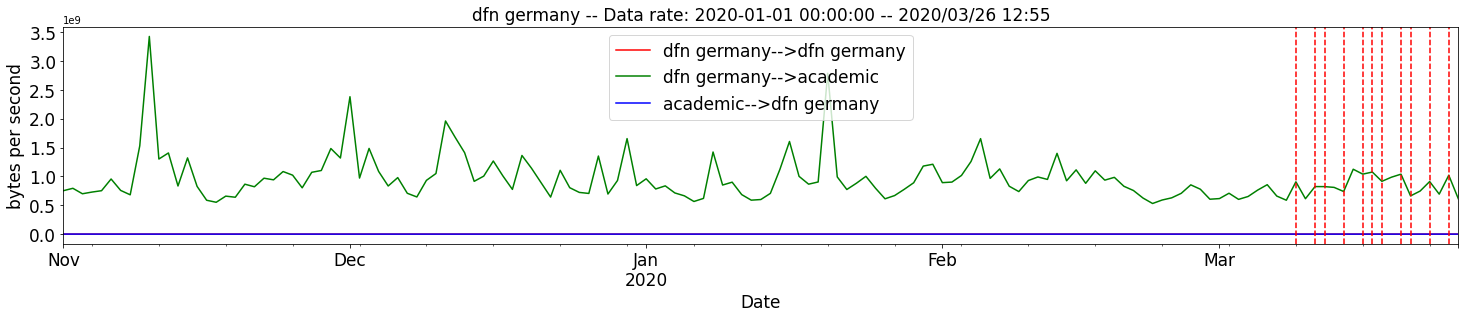
\includegraphics[width=\columnwidth]{img/dfn_aca_bps.png}
          \caption{DFN Germany}
          \label{fig:dfn_aca_bps}
    \end{subfigure}
    \begin{subfigure}{\linearFigSze\textwidth}
          \centering
          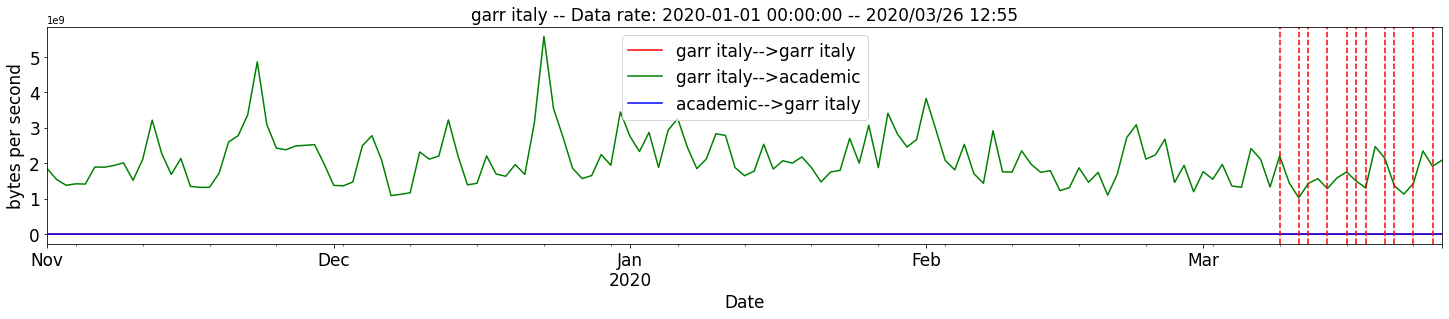
\includegraphics[width=\columnwidth]{img/garr_aca_bps.png}
          \caption{GARR Italy}
          \label{fig:garr_aca_bps}
    \end{subfigure}
    % \begin{subfigure}{\linearFigSze\textwidth}
    %       \centering
    %       \includegraphics[width=\columnwidth]{img/rediris_aca_fps.png}
    %       \caption{REDIRIS Spain}
    %       \label{fig:rediris_aca_fps}
    % \end{subfigure}
    % \begin{subfigure}{\linearFigSze\textwidth}
    %       \centering
    %       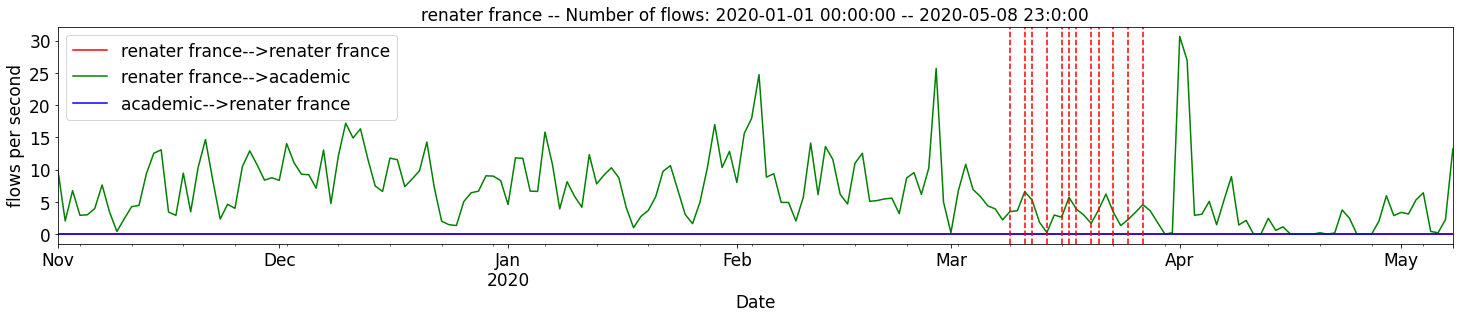
\includegraphics[width=\columnwidth]{img/renater_aca_fps.png}
    %       \caption{RENATER France}
    %       \label{fig:renater_aca_fps}
    % \end{subfigure}
    \begin{subfigure}{\linearFigSze\textwidth}
          \centering
          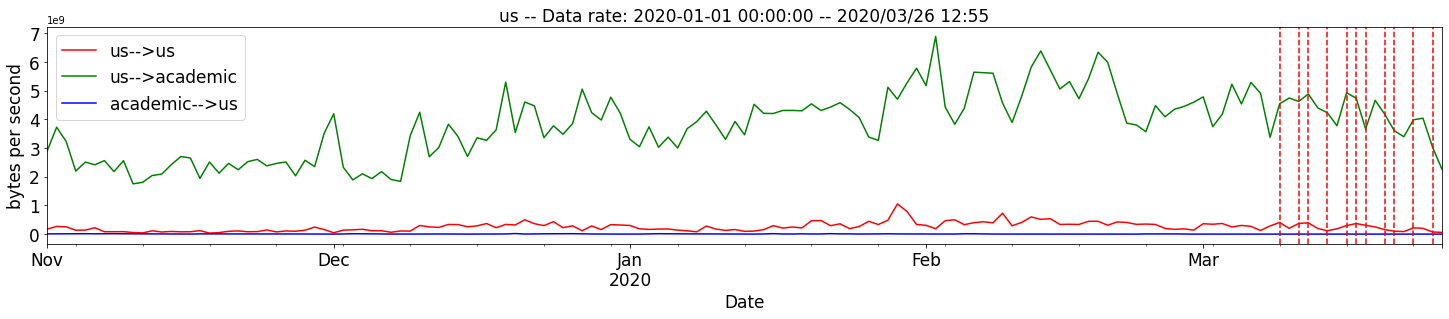
\includegraphics[width=\columnwidth]{img/us_aca_bps.png}
          \caption{US NREN}
          \label{fig:US_aca_bps}
    \end{subfigure}
    % \begin{subfigure}{\linearFigSze\textwidth}
    %       \centering
    %       \includegraphics[width=\columnwidth]{img/china_aca_fps.png}
    %       \caption{China NREN}
    %       \label{fig:china_aca_fps}
    % \end{subfigure}
    \caption{Traffic destined to Academic ASes of NRENs' (fps)}
    \label{fig:nrens_aca_bps}
\end{figure*}
\begin{figure*}
    \begin{subfigure}{\linearFigSze\textwidth}
          \centering
          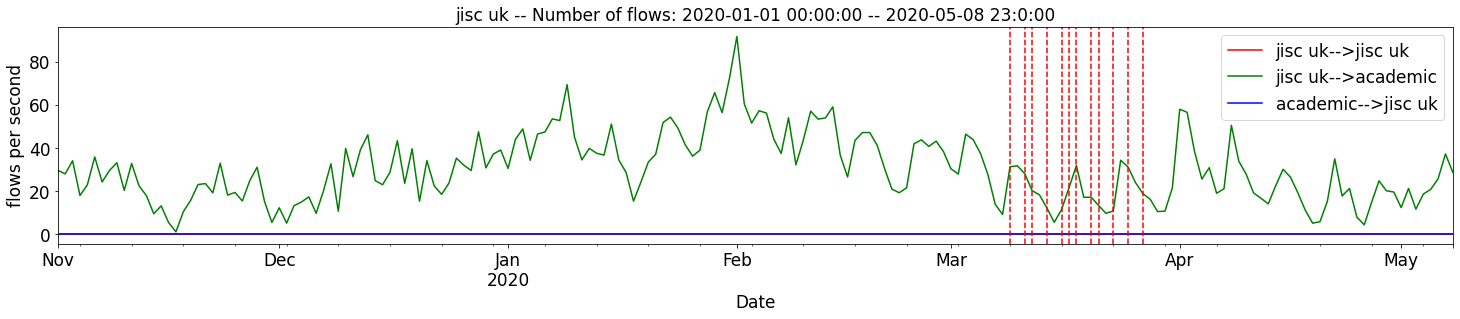
\includegraphics[width=\columnwidth]{img/jisc_aca_fps.png}
          \caption{JISC}
          \label{fig:jisc_aca_fps}
    \end{subfigure}
    % \begin{subfigure}{\linearFigSze\textwidth}
    %       \centering
    %       \includegraphics[width=\columnwidth]{img/heanet_aca_fps.png}
    %       \caption{HEANET}
    %       \label{fig:HEANET_aca_fps}
    % \end{subfigure}
    \begin{subfigure}{\linearFigSze\textwidth}
          \centering
          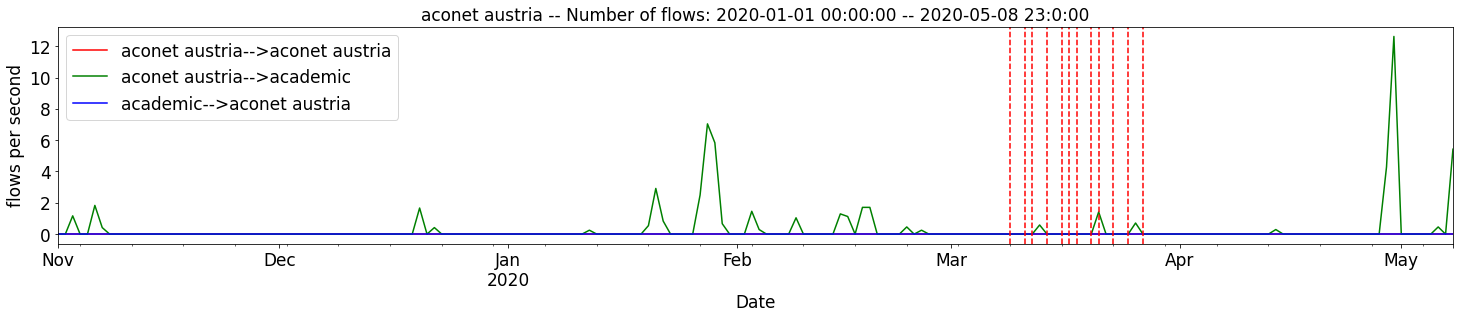
\includegraphics[width=\columnwidth]{img/aconet_aca_fps.png}
          \caption{ACONET Austria}
          \label{fig:aconet_aca_fps}
    \end{subfigure}
    \begin{subfigure}{\linearFigSze\textwidth}
          \centering
          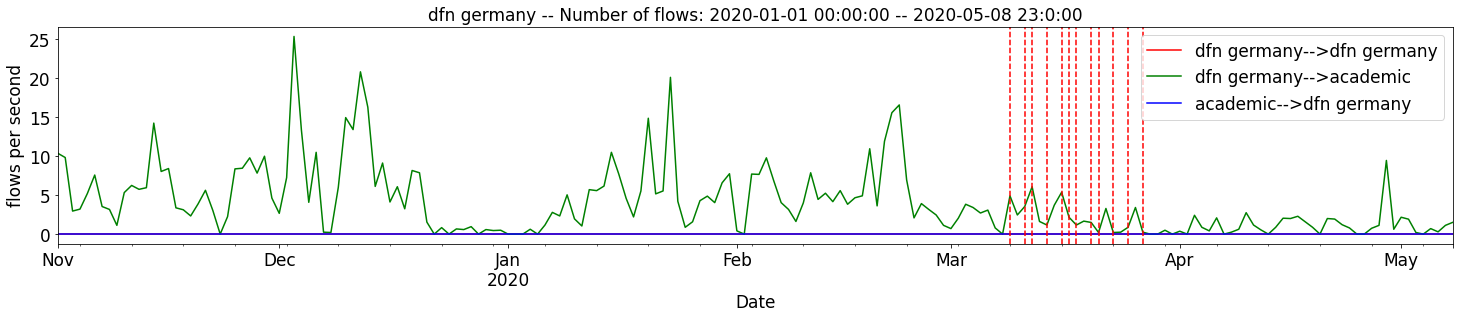
\includegraphics[width=\columnwidth]{img/dfn_aca_fps.png}
          \caption{DFN Germany}
          \label{fig:dfn_aca_fps}
    \end{subfigure}
    \begin{subfigure}{\linearFigSze\textwidth}
          \centering
          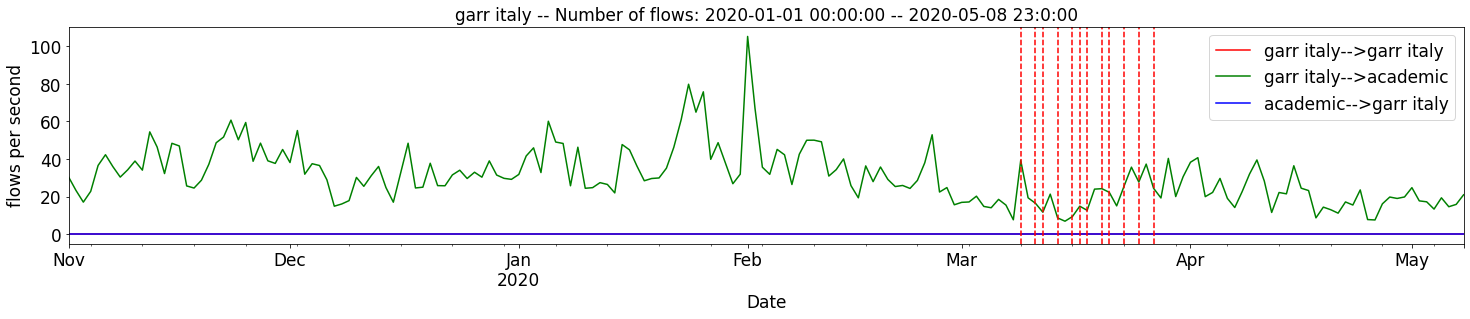
\includegraphics[width=\columnwidth]{img/garr_aca_fps.png}
          \caption{GARR Italy}
          \label{fig:garr_aca_fps}
    \end{subfigure}
    % \begin{subfigure}{\linearFigSze\textwidth}
    %       \centering
    %       \includegraphics[width=\columnwidth]{img/rediris_aca_fps.png}
    %       \caption{REDIRIS Spain}
    %       \label{fig:rediris_aca_fps}
    % \end{subfigure}
    % \begin{subfigure}{\linearFigSze\textwidth}
    %       \centering
    %       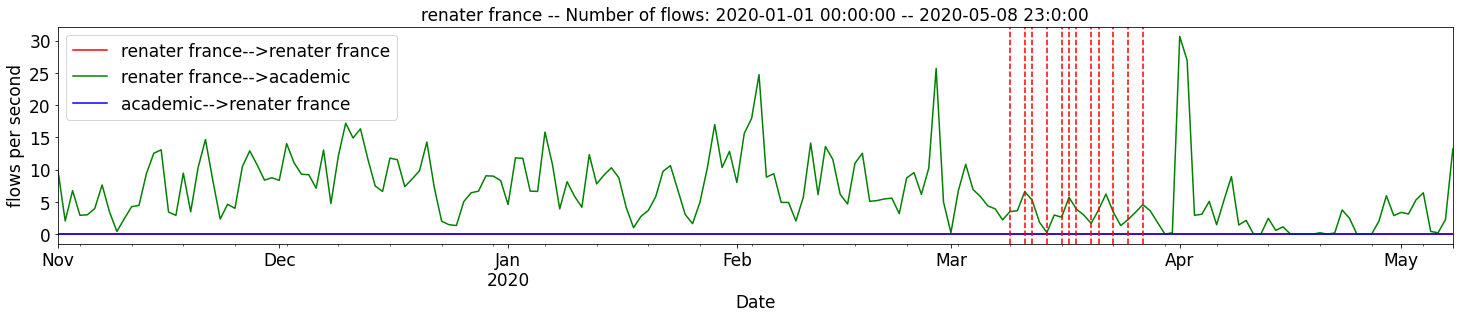
\includegraphics[width=\columnwidth]{img/renater_aca_fps.png}
    %       \caption{RENATER France}
    %       \label{fig:renater_aca_fps}
    % \end{subfigure}
    \begin{subfigure}{\linearFigSze\textwidth}
          \centering
          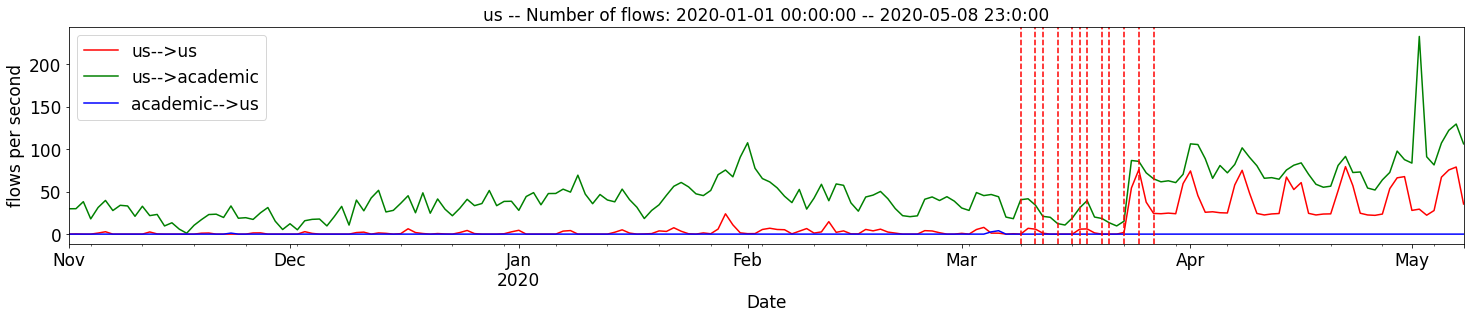
\includegraphics[width=\columnwidth]{img/us_aca_fps.png}
          \caption{US NREN}
          \label{fig:US_aca_fps}
    \end{subfigure}
    % \begin{subfigure}{\linearFigSze\textwidth}
    %       \centering
    %       \includegraphics[width=\columnwidth]{img/china_aca_fps.png}
    %       \caption{China NREN}
    %       \label{fig:china_aca_fps}
    % \end{subfigure}
    \caption{Traffic destined to Academic ASes of NRENs' (fps)}
    \label{fig:nrens_aca_fps}
\end{figure*}

\begin{figure*}
    \begin{subfigure}{\linearFigSze\textwidth}
          \centering
          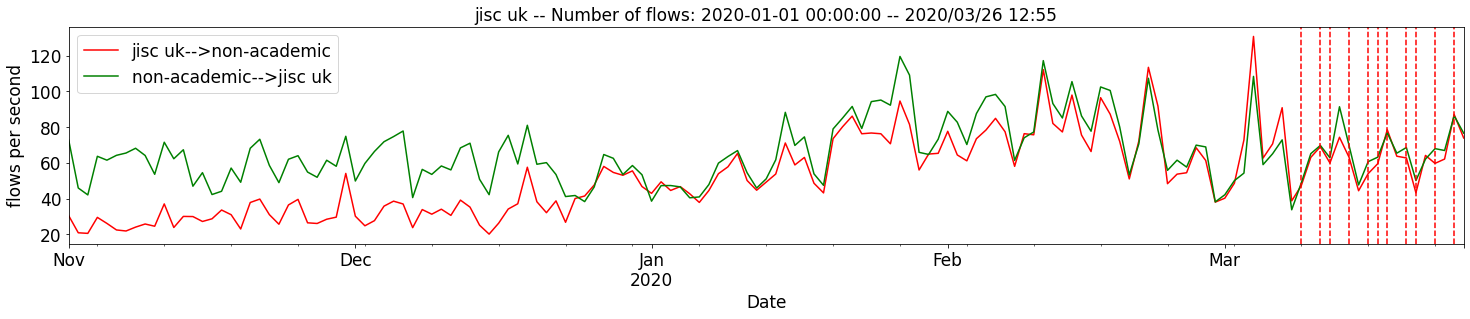
\includegraphics[width=\columnwidth]{img/jisc_busi_bps.png}
          \caption{JISC}
          \label{fig:jisc_busi_bps}
    \end{subfigure}
    % \begin{subfigure}{\linearFigSze\textwidth}
    %       \centering
    %       \includegraphics[width=\columnwidth]{img/heanet_busi_fps.png}
    %       \caption{HEANET}
    %       \label{fig:HEANET_busi_fps}
    % \end{subfigure}
    % \begin{subfigure}{\linearFigSze\textwidth}
    %       \centering
    %       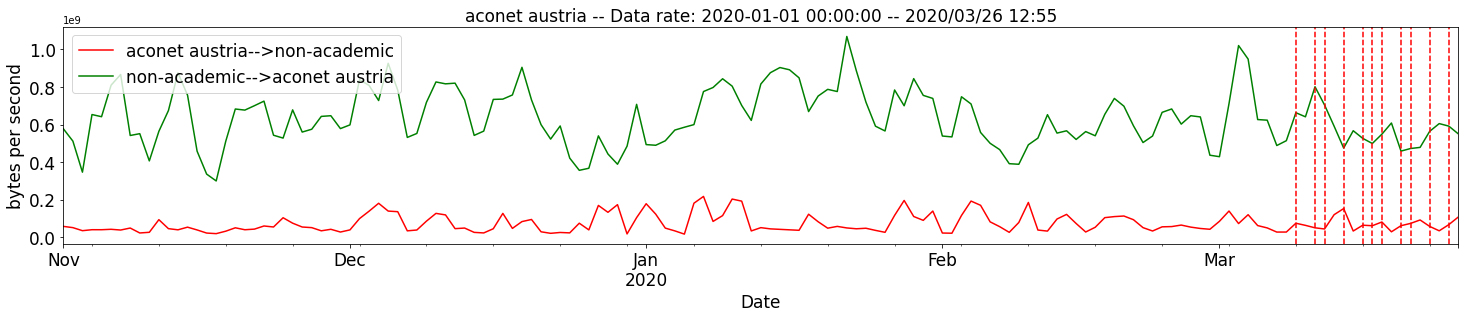
\includegraphics[width=\columnwidth]{img/aconet_busi_bps.png}
    %       \caption{ACONET Austria}
    %       \label{fig:aconet_aca_bps}
    % \end{subfigure}
    \begin{subfigure}{\linearFigSze\textwidth}
          \centering
          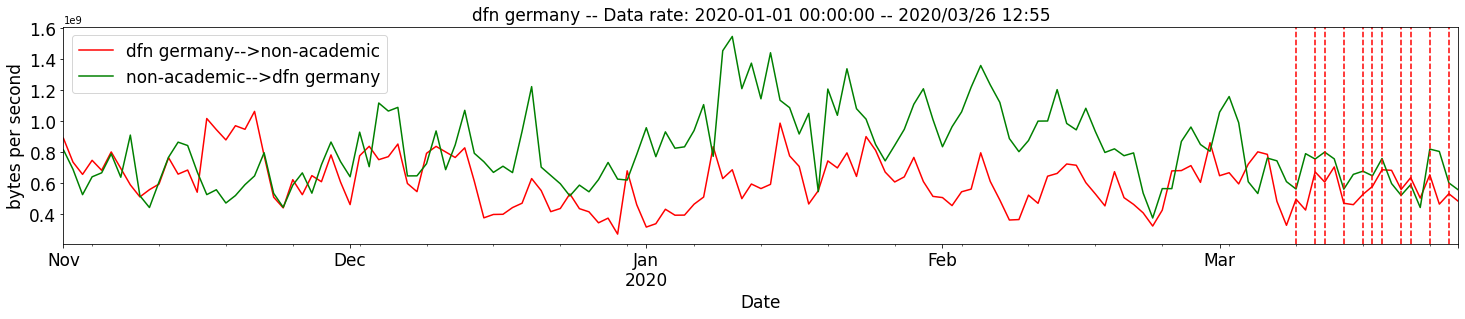
\includegraphics[width=\columnwidth]{img/dfn_busi_bps.png}
          \caption{DFN Germany}
          \label{fig:dfn_busi_bps}
    \end{subfigure}
    \begin{subfigure}{\linearFigSze\textwidth}
          \centering
          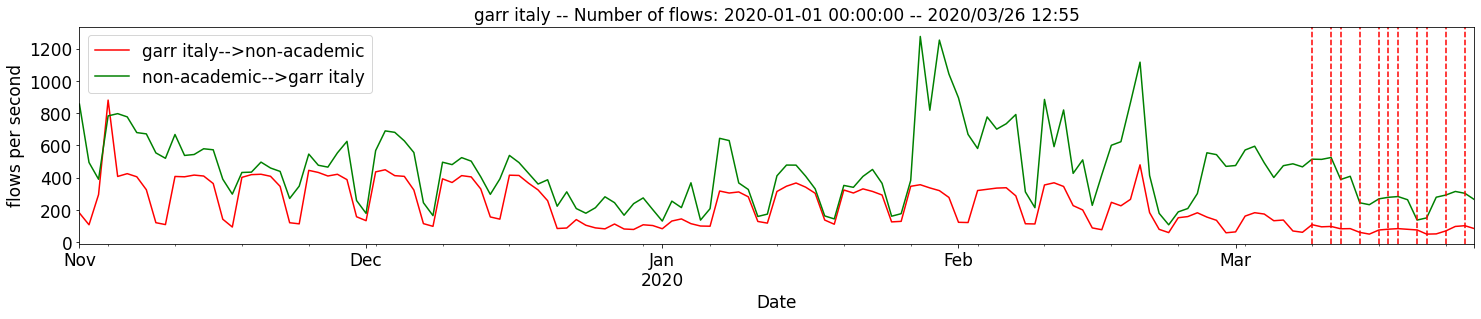
\includegraphics[width=\columnwidth]{img/garr_busi_bps.png}
          \caption{GARR Italy}
          \label{fig:garr_busi_bps}
    \end{subfigure}
    % \begin{subfigure}{\linearFigSze\textwidth}
    %       \centering
    %       \includegraphics[width=\columnwidth]{img/rediris_busi_fps.png}
    %       \caption{REDIRIS Spain}
    %       \label{fig:rediris_aca_fps}
    % \end{subfigure}
    % \begin{subfigure}{\linearFigSze\textwidth}
    %       \centering
    %       \includegraphics[width=\columnwidth]{img/renater_busi_fps.png}
    %       \caption{RENATER France}
    %       \label{fig:renater_aca_fps}
    % \end{subfigure}
    \begin{subfigure}{\linearFigSze\textwidth}
          \centering
          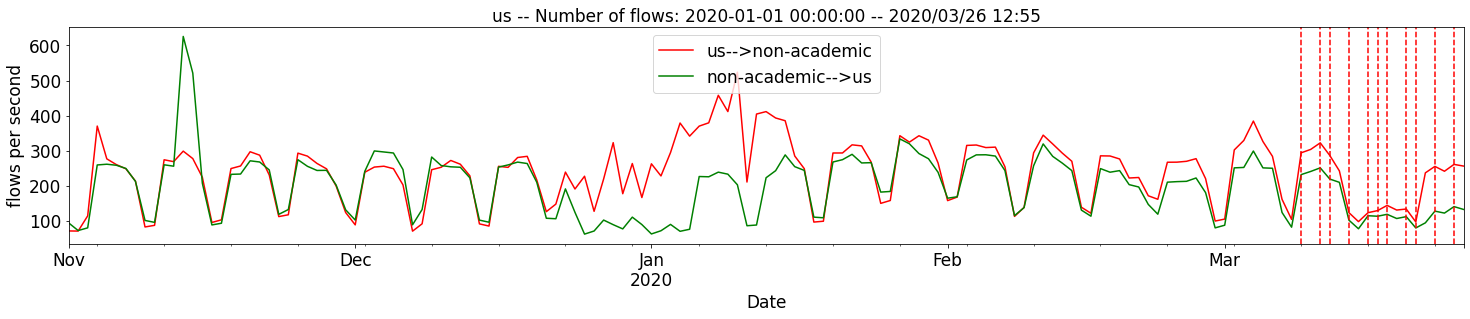
\includegraphics[width=\columnwidth]{img/us_busi_bps.png}
          \caption{US NREN}
          \label{fig:US_busi_bps}
    \end{subfigure}
    % \begin{subfigure}{\linearFigSze\textwidth}
    %       \centering
    %       \includegraphics[width=\columnwidth]{img/china_busi_fps.png}
    %       \caption{China NREN}
    %       \label{fig:china_aca_fps}
    % \end{subfigure}
    \caption{Traffic destined to Academic ASes of NRENs' (fps)}
    \label{fig:nrens_busi_bps}
\end{figure*}
\begin{figure*}
    \begin{subfigure}{\linearFigSze\textwidth}
          \centering
          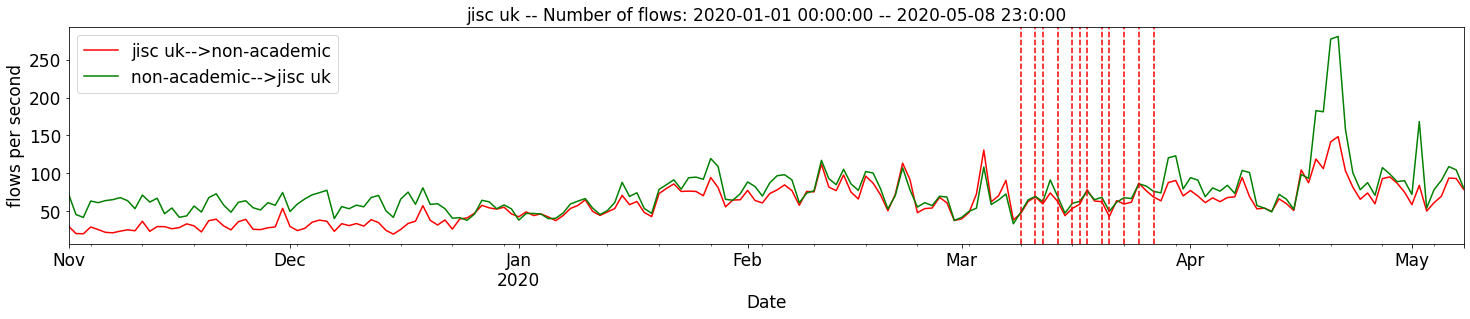
\includegraphics[width=\columnwidth]{img/jisc_busi_fps.png}
          \caption{JISC}
          \label{fig:jisc_busi_fps}
    \end{subfigure}
    % \begin{subfigure}{\linearFigSze\textwidth}
    %       \centering
    %       \includegraphics[width=\columnwidth]{img/heanet_busia_fps.png}
    %       \caption{HEANET}
    %       \label{fig:HEANET_busi_fps}
    % \end{subfigure}
    \begin{subfigure}{\linearFigSze\textwidth}
          \centering
          \includegraphics[width=\columnwidth]{img/aconet_busi_fps.png}
          \caption{ACONET Austria}
          \label{fig:aconet_busi_fps}
    \end{subfigure}
    \begin{subfigure}{\linearFigSze\textwidth}
          \centering
          \includegraphics[width=\columnwidth]{img/dfn_busi_fps.png}
          \caption{DFN Germany}
          \label{fig:dfn_busi_fps}
    \end{subfigure}
    % \begin{subfigure}{\linearFigSze\textwidth}
    %       \centering
    %       \includegraphics[width=\columnwidth]{img/garr_busi_fps.png}
    %       \caption{GARR Italy}
    %       \label{fig:garr_busi_fps}
    % \end{subfigure}
    % \begin{subfigure}{\linearFigSze\textwidth}
    %       \centering
    %       \includegraphics[width=\columnwidth]{img/rediris_busi_fps.png}
    %       \caption{REDIRIS Spain}
    %       \label{fig:rediris_aca_fps}
    % \end{subfigure}
    % \begin{subfigure}{\linearFigSze\textwidth}
    %       \centering
    %       \includegraphics[width=\columnwidth]{img/renater_busi_fps.png}
    %       \caption{RENATER France}
    %       \label{fig:renater_aca_fps}
    % \end{subfigure}
    \begin{subfigure}{\linearFigSze\textwidth}
          \centering
          \includegraphics[width=\columnwidth]{img/us_busi_fps.png}
          \caption{US NREN}
          \label{fig:US_busi_fps}
    \end{subfigure}
    % \begin{subfigure}{\linearFigSze\textwidth}
    %       \centering
    %       \includegraphics[width=\columnwidth]{img/china_busi_fps.png}
    %       \caption{China NREN}
    %       \label{fig:china_aca_fps}
    % \end{subfigure}
    \caption{Traffic destined to Academic ASes of NRENs' (fps)}
    \label{fig:nrens_busi_fps}
\end{figure*}

\subsection{histogram}

\begin{figure*}
    \begin{subfigure}{\histFigSze\textwidth}
          \centering
          \includegraphics[width=\columnwidth]{img/jisc_hist_fps.png}
          \caption{JISC}
          \label{fig:jisc_hist_fps}
    \end{subfigure}
    % \begin{subfigure}{\linearFigSze\textwidth}
    %       \centering
    %       \includegraphics[width=\columnwidth]{img/heanet_hist_fps.png}
    %       \caption{HEANET}
    %       \label{fig:HEANET_busi_fps}
    % \end{subfigure}
    \begin{subfigure}{\histFigSze\textwidth}
          \centering
          \includegraphics[width=\columnwidth]{img/aconet_hist_fps.png}
          \caption{ACONET Austria}
          \label{fig:aconet_hist_fps}
    \end{subfigure}
    \begin{subfigure}{\histFigSze\textwidth}
          \centering
          \includegraphics[width=\columnwidth]{img/dfn_hist_fps.png}
          \caption{DFN Germany}
          \label{fig:dfn_hist_fps}
    \end{subfigure}
    \begin{subfigure}{\histFigSze\textwidth}
          \centering
          \includegraphics[width=\columnwidth]{img/garr_hist_fps.png}
          \caption{GARR Italy}
          \label{fig:garr_hist_fps}
    \end{subfigure}
    \begin{subfigure}{\histFigSze\textwidth}
          \centering
          \includegraphics[width=\columnwidth]{img/rediris_hist_fps.png}
          \caption{REDIRIS Spain}
          \label{fig:rediris_hist_fps}
    \end{subfigure}
    \begin{subfigure}{\histFigSze\textwidth}
          \centering
          \includegraphics[width=\columnwidth]{img/renater_hist_fps.png}
          \caption{RENATER France}
          \label{fig:renater_hist_fps}
    \end{subfigure}
    \begin{subfigure}{\histFigSze\textwidth}
          \centering
          \includegraphics[width=\columnwidth]{img/us_hist_fps.png}
          \caption{US NREN}
          \label{fig:US_hist_fps}
    \end{subfigure}
    % \begin{subfigure}{\histFigSze\textwidth}
    %       \centering
    %       \includegraphics[width=\columnwidth]{img/china_hist_fps.png}
    %       \caption{China NREN}
    %       \label{fig:china_aca_fps}
    % \end{subfigure}
    \caption{Flow per Second Histogram}
    \label{fig:nrens_hist_fps}
\end{figure*}

\section{ASes}
\subsection{Top ASes fps and bps (box plot)}
\begin{figure*}
    \begin{subfigure}{\boxFigSze\textwidth}
          \centering
          \includegraphics[width=\columnwidth]{img/top_AS_generating_bps.png}
          \caption{Generating Traffic}
          \label{fig:top_generating_bps}
    \end{subfigure}
    \begin{subfigure}{\boxFigSze\textwidth}
          \centering
          \includegraphics[width=\columnwidth]{img/top_AS_receiving_bps.png}
          \caption{Receiving Traffic}
          \label{fig:top_receiving_bps}
    \end{subfigure}
    \caption{Top ASes (bps)}
    \label{fig:top_AS_bps}
\end{figure*}
\begin{figure*}
    \begin{subfigure}{\boxFigSze\textwidth}
          \centering
          \includegraphics[width=\textwidth]{img/top_AS_generating_fps.png}
          \caption{Generating Traffic}
          \label{fig:top_generating_fps}
    \end{subfigure}
    \begin{subfigure}{\boxFigSze\textwidth}
          \centering
          \includegraphics[width=\textwidth]{img/top_AS_receiving_fps.png}
          \caption{Receiving Traffic}
          \label{fig:top_receiving_fps}
    \end{subfigure}
    \caption{Top ASes (fps)}
    \label{fig:top_AS_fps}
\end{figure*}

\end{document}
